%-----------------------------------------------------------------------------
%
%               Template for sigplanconf LaTeX Class
%
% Name:         sigplanconf-template.tex
%
% Purpose:      A template for sigplanconf.cls, which is a LaTeX 2e class
%               file for SIGPLAN conference proceedings.
%
% Guide:        Refer to "Author's Guide to the ACM SIGPLAN Class,"
%               sigplanconf-guide.pdf
%
% Author:       Paul C. Anagnostopoulos
%               Windfall Software
%               978 371-2316
%               paul@windfall.com
%
% Created:      15 February 2005
%
%-----------------------------------------------------------------------------


\documentclass[preprint]{sigplanconf}

% The following \documentclass options may be useful:
%
% 10pt          To set in 10-point type instead of 9-point.
% 11pt          To set in 11-point type instead of 9-point.
% authoryear    To obtain author/year citation style instead of numeric.

\usepackage{amsfonts}
\usepackage{amsmath}
\usepackage{amsthm}
\usepackage{graphicx}
\usepackage{subfig}
\usepackage{epstopdf}
\usepackage{fancyvrb}
\usepackage{multicol}

\newtheorem{definition}{Definition}
\newtheorem{proposition}{Proposition}

\def\QED{\mbox{\rule[0pt]{1.5ex}{1.5ex}}}

\def\endproof{\hspace*{\fill}~\QED\par\endtrivlist}


\begin{document}

\conferenceinfo{PLDI '13}{June 16 -- 21, 2013, Seattle, Washington, USA.} 
\copyrightyear{2013} 
\copyrightdata{[to be supplied]} 

\titlebanner{banner above paper title}        % These are ignored unless
\preprintfooter{short description of paper}   % 'preprint' option specified.

\title{iMonitor: An Implicit-Signal Monitor Based on Predicate Tagging}
\subtitle{}

\authorinfo{Wei-Lun Hung\and Vijay K. Garg}
           {The University of Texas at Austin}
           {wlhung@utexas.edu, garg@ece.utexas.edu}

\maketitle

\begin{abstract}
For more than forty years, the parallel programming community has used monitor 
as the main mechanism for conditional synchronization. Most of the modern 
programming languages support only the explicit-signal monitor but the 
implicit-signal monitor due to the performance issues. In this paper, we 
argue that the implicit-signal monitor can be as efficient as implicit-signal
monitor or even more efficient for some examples.

To satisfy the need for implicit-signal monitor, we proposed a framework called 
iMonitor. tagging, relay guarantees, no signalAll. 

\end{abstract}

\category{CR-number}{subcategory}{third-level}

\terms
Algorithms, Languages, Performance 

\keywords
automatic signal, concurrency, explicit signal, implicit signal, monitor, 
parallel


% code examples







\section{Introduction} \label{sec:intro}
%Developing efficient and robust concurrent programs within a limited time is 
%critical than ever. On the one hand, the multi-core processor, which allows 
%multiple threads to be executed at the same time, has become the mainstream of 
%computers; however, the power of multi-core processors is limited due to the 
%lack of concurrent applications. In order to compete with other rivals
%and to satisfy consumers' demands in the software industry, applications need to be
%developed in a shot period. The concurrent programming is 
%different from the traditional sequential programming. Multiple threads may 
%interact with each other and try to access the same source. Form the programmers' perspective, 
%it is much more difficult to correctly develop concurrent programs than sequential programs. 
%In addition, the debugging process is panic in concurrent programs due to the 
%thread scheduling. 

%The monitor \cite{hoa74, han75} is commonly used in the concurrent programming for 
%maintaining the mutual exclusion of shared resources and providing the 
%synchronization mechanism between threads. Buhr and Harji \cite{bh05} divided 
%monitors into two categories, the explicit-signal monitor and the 
%implicit-signal monitor. Buhr and Harji used the explicit-signal monitor to 
%simulate the implicit-signal monitor and pointed out that the implicit-signal 
%monitor is not as efficient as the explicit-signal monitor. However, the 
%implicit-signal is easy to be used and useful in concurrent programming,
%especially for prototyping. 

%Most programming languages, including the popular object-oriented language Java,
%only provide the explicit-signal monitor but not implicit-signal. This research 
%focuses on developing a framework supporting implicit-signal monitor without
%sacrificing efficiency in the modern programming language - Java. 

%our contribution


The multicore hardware is now ubiquitous. Even the cell phones have
multicore processors. Programming these multicore processors is
still a challenging task due to
bugs resulted form concurrency and synchronization.
Although there is widespread acknowledgement of difficulties 
in programming these systems, it is almost hard to believe that 
by and large the most prevalent methods of dealing with synchronization are
based on ideas that were developed in early 70's \cite{hoa74, han75}. For 
example, the most widely used threads package in C++, pthreads, and
the most widely used package in Java, java.util.concurrent, are based
on the notion of monitors (or semaphores) developed in 60's and 70's.
In this research, we developed new method called iMonitor 
that allows gains in productivity of the programmer as well as gain in
performance of the system.

%\subsection{Why Is Implicit-Signal Monitor Needed?}
Both pthreads and Java require programmers to explicitly
signal threads that may be waiting on certain condition. The programmer
has to explicitly declare condition variables and then signal one
or all of the threads when the associated condition becomes true.
Using the wrong notification (signal versus signalAll) is a frequent
source of bugs. In iMonitor there is no notion of condition variables
and it is the responsibility of the system to signal appropriate threads.
This feature in iMonitor significantly reduces the program size and complexity.
Note that the idea of automatic signaling has been proposed 
in the original paper by Hoare as an alternative to implicit
signaling \cite{hoa74}. However, it is generally believed that implicit 
signaling is extremely inefficient compared to explicit signaling. 
For example, Buhu and Harji claim that implicit monitors are 10-50 times
slower than explicit signals \cite{bfc95}. The reason for the slowdown is that
previous implementations of implicit monitor are based on the
evaluation of all conditions, whenever monitor is available. 
We show in the paper that implicit signaling is still necessary for the 
following reasons:
\begin{enumerate}
    \item Potentially gaining performance through optimizing system based on
        architecture information and avoiding signalAll calls. A signalAll 
        call introduces unnecessary context switches and decreases performance. 
        The details will be given in Section \ref{sec:sigAll}.
    \item Less work for programmers, which implies fewer bugs in programs.
        In explicit-signal monitor, it is the responsibility of programmers to 
        explicitly invoke a signal call on some condition variable for
        conditional synchronization. Using the wrong notification or signaling
        a wrong condition variable are frequent source of bugs. 
    \item Violating separation of concerns. In explicit-signal monitor, the
        conditional synchronization is composed of two parts. A thread checks
        whether or not the condition has met and explicitly waits on a
        condition variable. Another thread detects the condition has met and
        explicit signal the condition variable. The intricate relation between
        threads for conditional synchronization leads the modularity of 
        programming and encapsulation difficult.  
    \item Mitigating the debugging of explicit-signal programs. It is easier to
        reason a implicit-signal code than a explicit-signal code. A correct
        implicit-signal implementation is helpful in debugging with a 
        explicit-signal implementation.  
    \item Rapid prototyping for speedup in developing process and accelerating
        products time to market.
\end{enumerate}

The relationship between the implicit-signal and explicit-signal monitor can be 
depicted by analogy with the relationship between the garbage collection and 
manual memory management. Although garbage collection leads to decreased
performance due to the overhead in deciding which memory to free; programmers 
elude manual memory deallocation. As a consequence, memory leaks and certain 
bugs, such as dangling pointer bugs and double free bugs, are reduced and 
eradicated. Similarly, implicit-signal mechanism consumes computing resources 
in deciding which thread to be signaled; programmers avoid explicitly invoking 
signal calls. As a result, some bugs, such as using wrong notification and
signaling a wrong condition variable, are diminished and eliminated. 
%\subsection{iMonitir Syntax}
%\subsection{iMonitor Example}
%The concurrent programs are more difficult to be written and debugged than the 
%sequential programs. Although explicit-signal monitor already provides an 
%elegant mechanism for programmers to maintain mutual exclusion and synchronization 
%in concurrent programs; implicit-signal is more straightforward in both code
%reasoning and syntax. 

To make the implicit-signal mechanism available in Java, we proposes the 
framework of iMonitor illustrated in Fig.~\ref{fig:fw}. In iMonitor, the 
programmer has to deal with fewer concepts and constructs than other monitors 
based on traditional methods. The iMonitor framework is composed of a 
preprocessor and a Java condition manager library. The preprocessor translates 
iMonitor codes into tradition Java codes. Our implicit-signal mechanism and 
developed techniques were implemented in the Java library. Although this paper 
focuses on only Java; our techniques are also applicable to other programming 
language, such as pthread and C\#.  

%Fig.~\ref{fig:fw} illustrates the framework of iMonitor, which makes 
%the implicit-signal available with the modern high-level language, Java. 
%The iMonitor takes a Java-extension program providing the implicit-signal 
%mechanism through supporting the monitor class and the waituntil statement. The 
%iMonitor preprocessor transfers an iMonitor code into the tradition Java code 
%that can be compiled with iMonitor library. The iMonitor 
%Java library implements our implicit-signal monitor mechanism.  
%
\begin{figure}[ht!]
  \centering
  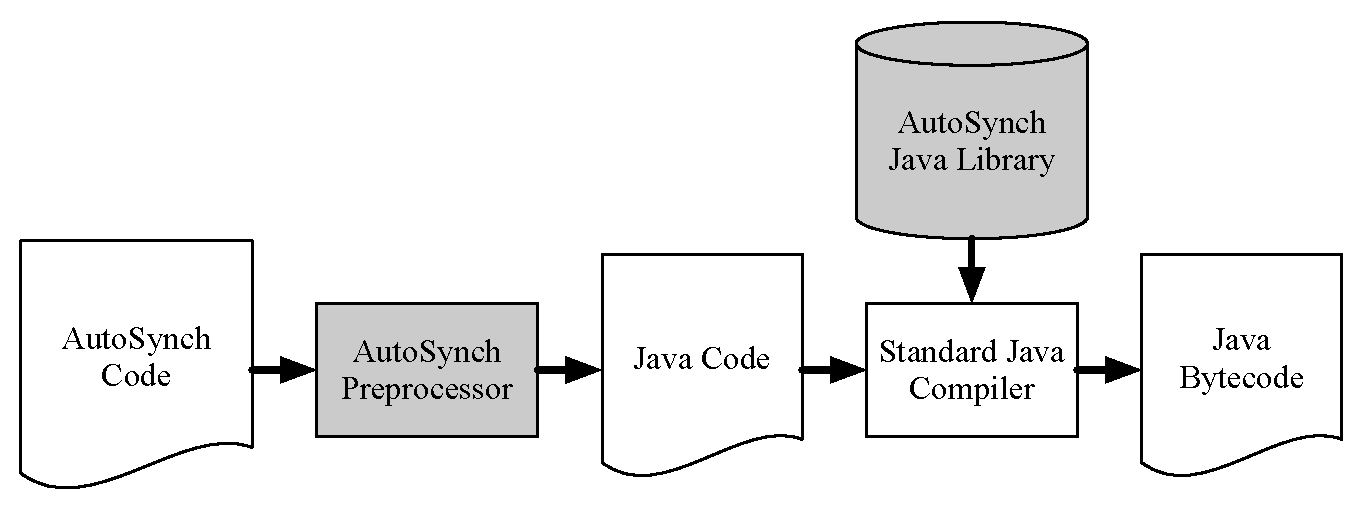
\includegraphics[width=80mm]{fig/flow.eps}
  \caption{The framework of iMonitor}
  \label{fig:fw}
\end{figure}


iMonitor extends Java with supporting the monitor class and the waituntil 
statement. A monitor class is defined as every member function of the class 
that can be executed by only one thread at any time. Namely, a monitor class is
mutual  exclusion by nature. The $monitor$ is reserved as a modifier, 
indicating a monitor class in iMonitor. A $waituntil$ statement, appearing in 
only member functions of a monitor class, has a predicate as its parameter. 
When a thread is executing a waituntil statement, it checks whether or not the 
predicate is true. The thread can continue to execute only when the predicate
is true. Otherwise, if the predicate is false, the executing tread must wait 
and release the privilege of the monitor control temporarily. 

Fig.~\ref{fig:bb_exp} shows an example demonstrating the difference between 
the Java implementation and the iMonitor implementation for the 
bounded-buffer problem, also known as the producer-consumer problem. 
In the problem, two kinds of threads, producers and consumers, tries to obtain 
access to the shared resources. Producers put items 
into the buffer, while consumers take items out from the buffer. Every 
operation should be mutual exclusion. Furthermore, a producer must wait  
when the buffer is full, while a consumer has to hold when the 
buffer is empty. The explicit-signal bounded buffer is written in Java. A 
lock variable and two condition variables are needed to maintain mutual exclusion 
and conditional synchronization. A thread needs to acquire the lock before entering member
functions. In addition, programmers need to explicitly associate conditional 
assertions with condition variables and call signal or await function manually.
On the contrary, 
the implicit-signal bounded buffer is written in our iMonitor framework.
Programmers use $monitor$ modifier to indicate the class is a monitor as line 
1. Besides, programmers use only $waituntil$ as in line 9 for conditional
synchronization. As can be expected, the implicit-signal monitor is
more straightforward and simpler than the explicit-signal monitor for
programmers in both code reasoning and syntax. 
\begin{figure*}[ht!]
\begin{multicols}{2}
    \begin{Verbatim}[fontsize=\footnotesize,gobble=8,frame=topline,
            framesep=5mm,numbers=left,numbersep=2pt,
            label=\fbox{\small\emph{Explicit-Signal}}]
        class BoundedBuffer {
          Object[] items;  
          int putPtr, takePtr, count;
          Lock mutex = new ReentrantLock();
          Condition notFull = mutex.newCondition();
          Condition notEmpty = mutex.newCondition();
          public BoundedBuffer(int n) {
            items = new Object[n];
            putPtr = takePtr = count = 0;
          }
          public void put(Object x) {
            mutex.lock();
            while (count == items.length) {
              notEmpty.signal();
              notFull.await();
            }
            items[putPtr++] = x;
            if (putPtr == items.length) {
              putPtr = 0;
            }
            ++count;
            notEmpty.signal();
            mutex.unlock();
          }
          public Object take() {
            mutex.lock();
            while (count == 0) {
              notFull.signal();
              notEmpty.await();
            }
            int x = items[takePtr];
            if (takePtr == items.length) {
              takePtr = 0;
            }
            --count;
            notFull.signal();
            mutex.unlock();
            return x;
          }
        }
    \end{Verbatim}
    \begin{Verbatim}[fontsize=\footnotesize,gobble=8,frame=lines,framesep=5mm,
            numbers=left,numbersep=2pt,
            label=\fbox{\small\emph{Implicit-Signal}}]
        monitor class BoundedBuffer { 
          Object[] items; 
          int putPtr, takePtr, count; 
          public BoundedBuffer(int n) {
            items = new Object[n];
            putPtr = takePtr = count = 0;
          }
          public void put(Object x) { 
            waituntil(count < items.length); 
            items[putPtr++] = x; 
            if (putPtr == items.length) { 
              putPtr = 0; 
            } 
            ++count; 
          } 
          public Object take() { 
            waituntil(count > 0); 
            Object x = items[takePtr++]; 
            if (takePtr == items.length) { 
              takePtr = 0; 
            }
            --count;
            return x;
          }
        }
    \end{Verbatim}
\end{multicols}
  \caption{Bounded-buffer example}
  \label{fig:bb_exp}
\end{figure*}

%\subsection{Design Principles}
In this paper we argue that implicit signaling is generally as fast as explicit 
and even faster for some examples. In Section \ref{sec:sigAll}, we give reasons
for the efficiency in implicit signaling. In short, the explicit signaling has 
to resort to signalAll in some examples; however, our implicit signaling never 
uses signalAll. We hope to design and build iMonitor that is almost always as 
fast as explicit and considerably faster for synchronization problems with 
signalAll. The design principles underlying iMonitor are as follows.

\begin{description}
    \item{\bf Reduce context switches.} Context switch requires a certain 
        amount of time to save and load registers and update various tables and
        lists. Reducing unnecessary context switches boosts the performance.
        A signalAll call introduces unnecessary context switches; therefore,
        signal calls are forbidden in iMonitor. 
    \item {\bf Check less predicates, if possible.} In the implicit-signal
        mechanism, automatically signaling a thread is the responsibility of our
        system. Checking less predicates to signal an appropriate thread is
        desired. 
\end{description}



%\subsection{Contributions}
The starting point in the design of iMonitor is how to evaluate predicates of
waituntil statements. Any thread that can access a monitor can check all 
predicates of waituntil statements of the monitor. Therefore, a thread can 
decide to signal another thread with a true predicate before the thread waits
or exits the monitor. We investigated globalization operation to eable 
predicate evaluations in any thread. Based on this operation, our framework can
provides relay guarantee and accelerate the process in deciding which thread to
be signaled with predicate tagging. To avoid using signalAll call, iMonitor 
provids relay guarantee, which ensures that some waiting thread with a true 
predicate is always signaled. Furthermore, predicate tags are used to
classify predicates. In deciding which thread should be signaled, after
examining the current state of a monitor, we can know which tags are infeasible
to be true at the moment. Then we only need to check the predicates without
those tags. 

Our experimental results indicate that iMonitor can significantly improve
performance \dots

Our main contributions are as follows.
\begin{enumerate}
    \item Presents the design and implementation of the iMonitor framework,
        which supports concurrent programs with implicit-signal mechanism.
    \item Experimental evaluation of iMonitor showing significant
        improvements in performance and scalability with predicate tagging
        and relay guarantee. 
    \item Experimental evidence indicating that iMonitor's implicit-signal
        mechanism is almost as efficient as explicit-signal mechanism or even 
        more efficient with much simpler code complexity.
\end{enumerate}
%In this project, we are developing multiple such features.
%Our second goal for SuperSynch is that the performance of the system
%with SuperSynch is at least as good as that for traditional systems.
%Continuing with the previous example of signaling threads,
%it is easy to develop automatic signaling mechanisms if performance
%is not an issue. For example, one could evaluate conditions for all
%threads. However, such a system would be significantly slower
%than explicit signaling systems for most programs. In this project
%we are developing techniques that usually result in programs
%with automatic signaling that are faster than the programs
%with explicit signaling. Thus, we get simpler programs with 
%faster performance. 

%Another aspect we are investigating in SuperSunch is the 
%idea of abortable monitor methods. The abortable methods 
%will support two widely used and familiar methods of programming
%(but not supported either by pthreads or Java). The 
%first notion is that of abortable transactions used in databases
%for decades. Although the concept has now entered in concurrent programming world 
%via transactional memories
%\section{Design of iMonitor} \label{sec:fw}


%\subsection{Organization}
This paper is organized as follows. Section \ref{sec:bg} gives the background
of montior. 
Section \ref{sec:sigAll} explains why signalAll is essential but bad. Our 
concepts are presented in Section \ref{sec:concept} and the practical 
implementation details are discussed in Section  \ref{sec:imp}. The proposed 
methods are then evaluated with experiments in Section \ref{sec:eval}. 
Our results are contrasted with prior work in Section \ref{sec:related}. 
Section \ref{sec:conclu} gives the concluding remarks.

\section{Background: monitor} \label{sec:bg}
%\subsection{Monitor}
Monitor is an abstract object or module containing shared data to be used safely
by multiple member functions and threads in concurrent programming. Monitor can
be defined by two characteristics, mutual exclusion and conditional 
synchronization. Mutual exclusion guarantees that at most one thread can 
execute any member function of a monitor at any time. It provides programmers a 
more elegant way to update shared data when compared to other access mechanism
such as semaphore. In general, threads need to acquire the lock of a monitor 
to acquire the privilege for accessing the monitor. Conditional synchronization 
maintains the executing order between threads. Threads may wait for some 
condition to be met and release the monitor lock temporarily. After the 
condition has been met, threads then re-acquire the lock and continue to 
execute. According to Buhr and Harji \cite{bh05}, monitors can be divided into 
two categories according to the different implementations of conditional 
synchronization. 
\begin{description}
    \item{\bf Explicit-signal monitor} In this type of monitor, condition
    variables, signal and await functions are used for synchronization. 
    Programmers need to associate assertions with condition variables manually.
    This mechanism involves two threads. One tread checks if some
    assertion is met or not, and then explicit waits on some condition variable 
    if the assertion is not met. When another thread detects that the state has 
    changed and the assertion is met, and then explicitly signals the 
    appropriate condition variable for waking threads.
    \item{\bf Implicit-signal monitor} This kind of monitor uses waituntil
    statements, such as line 9 in implicit-signal program in
    Fig.~\ref{fig:bb_exp}, instead of condition variables for
    synchronization. Programmers do not need to associate assertions with
    variables, but use waituntil statements directly. In
    monitor, a thread will wait if the condition of a waitutil
    statement is false, and execute the remaining tasks after the condition 
    becomes true. The responsibility of signaling the waiting thread is the
    system rather than the programmers. 
\end{description}

Obviously, the explicit-signal is more complex than the implicit-signal monitor 
for programmers. The explicit-signal requires that programmers
have to write their conditional synchronization manually, which increases the 
chance of writing incorrect code. The major advantage of the explicit-signal
monitor is the performance. It is generally believed that that explicit-signal 
monitor is much faster than the implicit-signal monitor. In this paper, we 
argue that the implicit-signal monitor could be as efficient as the
explicit-signal or ever faster in some cases. 

\section{Why is signalAll essential but bad?} \label{sec:sigAll}
The signalAll call is essential in explicit-signal mechanism when programmers
do not know which thread should be signaled. Fig.~\ref{fig:sigAll_exp}
illustrates an example. This example is also a bounded-buffer problem but 
different from Fig.~\ref{fig:bb_exp}. In this example, a producer can put 
$n$ items to the buffer a time, while a consumer can take $n$ items from the 
buffer a time. Furthermore, a producer must wait if there is no space to put
$n$ items, while a consumer has to hold when the buffer has insufficient items.
The signalAll calls should be used instead of signal calls. The reason is that
every producer and consumer waits for different condition to be met;
programmers do not know which producer or consumer should be signaled at
runtime. Although programmers can avoid using signalAll calls by writing
complicated code that associates different predicates to different condition 
variables; the complicated code makes the program difficult to be reasoned and 
maintained. 

The signalAll call is bad since it may decreases the performance. The reason is 
that signalAll calls introduce redundant context switches, requiring a certain 
computing time to save and load registers and update various tables and lists.
Furthermore, signalAll calls cannot increase parallelism because that threads
are forbidden to access a monitor simultaneously. Although multiple threads are
signaled at a time, only one thread is able to acquire the monitor. Many other 
threads need to go back to waiting state since another thread may change the 
status of the monitor. For example, the buffer has 64 items after a producer 
finishes a put call. The producer calls $insufficientItem.signalAll()$ as in 
line 24 before completing the call. Two waiting consumers are signaled; the 
consumer $C_1$ is waiting to take $48$ items while the consumer $C_2$ is 
waiting to take 
$32$ items. Suppose $C_1$ re-acquires the lock first and takes $48$ items. The
remaining items are $16$. Then $C_2$ re-acquires the lock; it figures out that
the items are insufficient and then goes back to waiting state. Waking $C_2$ is
redundant since it does not make any progress but go back to waiting.
Therefore, if we avoid using the signalAll call and only signal a thread which
is mostly like to make progress, the unnecessary context switches then can be
reduced.

\begin{figure}[ht!]
    \begin{Verbatim}[fontsize=\footnotesize,gobble=8,frame=lines,
            framesep=5mm,numbers=left,numbersep=2pt,
            label=\fbox{\small\emph{Explicit-Signal}}]
        class BoundedBuffer {
          Object[] items;  
          int putPtr, takePtr, count;
          Lock mutex = new ReentrantLock();
          Condition insufficientSpace = mutex.newCondition();
          Condition insufficientItem = mutex.newCondition();
          public BoundedBuffer(int n) {
            items = new Object[n];
            putPtr = takePtr = count = 0;
          }
          public void put(int n) {
            mutex.lock();
            while (n + count > items.length) {
              insufficientItem.signalAll();
              insufficientSpace.await();
            }
            for (int i = 0; i < n; ++i) {
              items[putPtr++] = new Object();
              if (putPtr == items.length) {
                putPtr = 0;
              }
            }
            count += n;
            insufficientItem.signalAll();
            mutex.unlock();
          }
          public Object[] take(int n) {
            mutex.lock();
            while (count < n) {
              insufficientSpace.signalAll();
              insufficientItem.await();
            }
            Object[] ret = new Object[n];
            for (int i = 0; i < n; ++i) {
              ret[i] = items[takePtr++];
              if (takePtr == items.length) {
                takePtr = 0;
              }
            }
            count -= n;
            insufficientSpace.signalAll();
            mutex.unlock();
            return ret;
          }
        }
    \end{Verbatim}
    \caption{Bounded-buffer* example}
    \label{fig:sigAll_exp}
\end{figure}


\section{iMonitor concepts} \label{sec:concept}


\subsection{Predicate evaluation}
%In order to allow any thread that can access a monitor to evaluation all
%predicates of waiting threads, an operation called globalization is defined as 
%replacing all local variables of
%a predicate by its values at the time. The globalization converts a local 
%predicate into a global predicate since all the local variables have been 
%replaced. The globalization has an important characteristic that allows a
%local predicate to be evaluated by any other thread safely after the original
%thread waits. The reason is that no other thread can access to the local variables of a member 
%function in which a particular thread is executing; therefore values of local variables 
%cannot be changed by other threads after a particular thread is waiting. 
%All other threads can check the globalized predicate safely. 
%\subsection{Predicate}
In iMonitor, it is the responsibility of the system to signal appropriate 
threads automatically. The predicate evaluation is crucial in deciding which
thread should be signaled. We will discuss how to preform predicate evaluations
of waituntil statements. 

A predicate $P(\vec{x}): X \rightarrow \mathbb{B}$ is a Boolean condition, 
where $X$ is the space spanned by the variables $\vec{x}=(x_1, \dots, x_n)$. 
A variable of a monitor object is a shared variable if it is accessible to every 
threads that accessing the monitor. The set of shared variables, denoted by 
$S$. On the contrary, the set of local variables, denoted by $L$, is only 
accessible by a thread calling a function in which the variables are declared. 

Predicates can be used to describe the properties of conditions. In this paper,
the predicate is used to depict the condition of every waituntil statement. 
Furthermore, we assume that every predicate, $p = \sum_i^nc_i$, is disjunctive 
normal form (DNF), where $c_i$ is defined as the conjunction of a set
of atomic Boolean expressions. Every Boolean formulas can be converted into DNF 
using De Morgan's laws and distributive law. 

Predicates can be divided into two categories based on the type of their 
depending variables \cite{bh05}.
\begin{definition}
    Consider a predicate $P(\vec{x}): X \rightarrow \mathbb{B}$. If $X 
    \subseteq S$, $P$ 
    is a restricted predicate. Otherwise, if $X \not\subseteq S$, $P$ 
    is a general predicate. 
\end{definition}

Evaluating a general predicate in all threads is unattainable 
because the accessibility of the local variables in the predicate is limited 
to the thread declaring them. To evaluate a general predicate in all 
threads, we treat local variables as constant values at runtime and define 
globalization as follows. 
\begin{definition}
    Given a general predicate $P(\vec{x}, \vec{y}): X \times Y \rightarrow 
    \mathbb{B}$, where $X \subseteq S$ and $Y \subseteq L$. The globalization 
    of $P$ at runtime $t$ is the new restricted predicate
    \[
    G_t(\vec{x}) = P(\vec{x}, \vec{y_t}),
    \]
    where $\vec{y_t}$ the values of $\vec{y}$ at runtime $t$.
\end{definition}
\begin{proposition} \label{pro:glob}
    Consider a general predicate $P(\vec{x}, \vec{y})$ in a waituntil 
    statement. $P(\vec{x}, \vec{y})$ and its globlization 
    $P(\vec{x}, \vec{y_t})$ are semantically equivalent during the waituntil 
    period, where $t$ is the runtime immediately before invoking the 
    waituntil statement.  
\end{proposition}
\begin{proof}
    Only the thread invoking the waituntil statement is able to access the
    local variables of the predicate; all other threads are unable to change
    the values of those local variables. Therefore, $\vec{y}$ is constant 
    during the waituntil period. Since $\vec{y_t}$ is the value of $\vec{y}$
    immediately before invoking the waituntil predicate, $P(\vec{x}, \vec{y})$
    and $P(\vec{x}, \vec{y_t})$ are semantic equivalent during the waituntil
    statement. 
\end{proof}

Proposition \ref{pro:glob} enables the general predicate evaluation of
waituntil statement in all threads. 
Given a general predicate in a waituntil statement, in the sequel we substitute
all the local variables with their values immediately before invoking the
statement. The predicate can be evaluated in all other threads during the
waituntil period. 

\subsection{Relay guarantee}
As mentioned in Section ~\ref{sec:sigAll}, signalAll calls are inevitable in
the explicit-signal mechanism sometimes; however, signalAll calls may decrease
performance by introducing redundant context switches. 
In
iMonitor, signalAll calls are avoided by providing the following guarantee. 
%should be reduced. Before a waiting thread is signaled, the 
%predicate of the waiting thread is ensured to be true. In addition, at most 
%one waiting thread is signaled at any time. The reason is that threads are 
%forbidden to access a monitor simultaneously. Signaling multiple threads does 
%not increase parallelism but redundant context switches. 

\begin{definition}{Relay guarantee:}
    when a thread exits a monitor or goes into waiting state, it checks whether
    or not there is some thread waiting on a condition which has been met. If
    at least one such waiting thread exists, the thread then signal one such
    waiting thread.
\end{definition}
\begin{proposition} \label{pro:one}
    Relay guarantee never introduces deadlock. That is,
    some waiting thread with true predicates are always signaled. 
\end{proposition}
\begin{proof}
    Suppose not. All waiting threads with true predicates are blocked and 
    no other thread can signal them. Consider a true predicate $P$. Since some
    thread goes into waiting state with $P$, $P$ is false initially. Some 
    other threads must enter the monitor and change the status of the monitor 
    to make $P$ true. Suppose thread $T$ is the last thread active 
    in the monitor. Since $P$ has become true, $T$ must signal one thread
    waiting on $P$ or other true predicate before leaving or 
    going into waiting state. A contradiction. 
 \end{proof}

Proposition \ref{pro:one} lays the theoretical foundation that signalAll calls
are avoidable by providing relay guarantee. Every time a
thread exits a monitor or goes into waiting state, it checks whether a
waiting thread has a true predicate. If at least one waiting thread has true
predicate, then one such thread is signaled. The remaining problem is how to 
find such thread efficiently. 

\subsection{Predicate tag}
In order to find an appropriate thread with a true predicate efficiently, 
different tags are assigned to every predicate according to its semantics. 
Those tags depict the properties of a predicate and allow true predicates to be 
found efficiently by examining the state of a monitor. Before going through the 
details, two particular types of predicates are defined as follows according to
the their semantics. 
\begin{definition}
    A predicate $P: (v = c)$ is an equivalence predicate, where $v \in S$ is 
    the pivot variable, and either $c \in L$ or $c$ is a constant 
    value.
\end{definition}
%\begin{definition}
%    A predicate $P: (v \neq c)$ is a non-equivalence predicate, where $v$ is the
%    pivot variable and $v \in S$, and either $c \in L$ or $c$ is a constant 
%    value.
%\end{definition}
\begin{definition}
   A predicate $P: (v\ \boldsymbol{op}\ c)$ is a threshold predicate, where 
   $\boldsymbol{op}
    \in \{<,\ \le,\ >,\ \ge\}$, $v \in S$ is the pivot variable, and 
    either $c \in L$ or $c$ is a constant value.
\end{definition}
These two types of predicates are XX\%. 

In general, tags are assigned to predicates according to their types. The 
formal definition of the tag is as follows. 
\begin{definition}
   A tag $T$ is a four-tuple $(M, op, v, c)$, where  
   \begin{itemize}
      \item $M \in \{Equivalence,\ Threshold,\ None\}$;
      \item $op \in \{<,\ \le,\ >,\ \ge\}$ if $L = Threshold$; otherwise, 
         $op = \perp$;
      \item $v$ and $c$ are the name of pivot variable and the constant
         value if $L \in \{Equivalence,\ Threshold\}$; otherwise, $v = \perp$
         and $c = \perp$.
   \end{itemize}
\end{definition}
Every $Equivalence$ or $Threshold$ tag represents a equivalence predicate or
threshold predicate respectively. We say a tag is true if the predicate
represented by the tag is true; otherwise, we say the tag is false. 
\subsubsection{Predicate tagging}
Tags are given to every predicate by the algorithm shown in
Fig.~\ref{fig:tagging}. The tags of conjunctions of a predicate form the set of 
tags of the predicate. A tag is assigned to every conjunction. When assigning a 
tag to a conjunction, the equivalence tag has higher priority than others. The
reason is that an equivalence predicate is more deterministic than a threshold 
predicate since the predicate is true only when the value of its pivot variable 
equal a specific value. For example, consider a equivalence predicate $x = 8$
and a threshold predicate $x > 3$. $x = 8$ is true only when the value of $x$
is $8$. On the contrary, $x > 3$ is true for every value of $x$ is greater than
$3$. Therefore, the $Equivalence$ tags is more helpful in
pruning false predicates than other kinds of tags. If a conjunction does not 
include any equivalence predicate, then we check whether or not it 
include any threshold predicate. If yes, then a $Threshold$ tag is assigned 
to the conjunction; otherwise, the conjunction has $None$ tag. 

Creating all tags for a conjunction is unnecessary. If a conjunction includes 
multiple equivalence predicates or threshold predicates, only one arbitrary 
$Equivalence$ tag or threshold tag is assigned to the clause. The first reason is 
that, if there is a large number of tags, then the performance may decrease due 
to cost of maintaining tags. The second reason is that the motivation behind 
the tag is to accelerate the searching process by pruning false predicate 
but not exhaustive search.  A clause is false when at least one 
of its atomic Boolean expressions is false. A tag of a clause is sufficient to 
help us in pruning this predicate when it is false. For example, consider a
conjunction $(x = 8) \wedge (y = 9)$. Only tag $(Equivalence,\ null,\ x,\ 8)$
is assigned to the conjunction. We check the predicate only when the tag is
true. Adding another tag $(Equivalence,\ null,\ y,\ 9)$ cannot help us in pruning
this predicate when it is false since we need to check both tags. Hence, we 
creating only one tag for each conjunction.
 
\begin{figure}[ht!]
    \begin{Verbatim}[fontsize=\footnotesize,gobble=8,frame=lines,
            framesep=3mm]
         tags = empty
         foreach conjunction c 
         if c contains an equivalence predicate x=v
            tag t = (Equivalence, null, x, v)
            add t to tags
         else if c contains a threshold predicate x op v
            tag t = (Threshold, op, x, v)
            add t to tags
         else 
            tag t = (None, null, null, null)
            add t to tags
         return tags
    \end{Verbatim}
  \caption{Predicate Tagging}
  \label{fig:tagging}
\end{figure}


\subsubsection{Tag signaling}
Signaling mechanism in iMonitor is based on tags. 
Since the equivalence tag is more deterministic than the threshold tag, the
predicates with equivalence are checked prior to the predicates with other 
tags. If no true predicate can be found after examining $Equivalence$ tags and
$Threshold$ tags, our algorithm does the exhaustive search for the predicates 
with $None$ tags. 

\paragraph{Equivalence tag signaling}
Observes that, an equivalence predicate becomes true only when its pivot 
variable equals the specific value in the predicate. For distinct equivalence 
tags related to a same pivot variable, at most one tag can be true at a time 
because the value of pivot variable is deterministic and unique at any time. By 
observing the value of the pivot variable, the appropriate tag can be 
identified if there is any. For example, there are three $Equivalence$ tags for
predicates $x = 3$, $x = 6$, and $x = 8$. We examine $x$ and figure out that
its value is $8$. Then we know that only $x = 8$ is true. Based on this 
observation, for each unique pivot variable of an equivalence tag, we create a 
hash table, where the specific value is used as the key. By using this hash 
table and examining the value of the pivot variable at runtime, we can decide a
true tag in $O(1)$ time if there is any. Then we only need to check the 
predicates with the tag. 

%Monotonic predicate evaluations can be optimized by the following observation. 
%\subsubsection{Non-Equivalence Predicate Signaling}
%Observing that, the value of a variable is deterministic and unique at any 
%time. Two distinct non-equivalence predicates with a same pivot variable cannot
%be false simultaneously. For example, at least one of $x \ne 8$ and $x \ne 5$
%is true. Non-equivalence predicates with a same pivot variable are stored in
%a linked list. By checking the first two predicates of the 
%linked list, at least one predicate is true. 

\paragraph{Threshold tag signaling}
For threshold tag, we consider the following situation. Suppose there are two 
predicates, $x > 5$ and $x > 3$, we know that if $x > 3$ is false, and then 
$x > 5$ cannot be true. That is, we only need to check the predicate with the 
smallest threshold value for $>$ and $\ge$ operations. Furthermore, consider the predicates
with the same threshold value but different operations, $x > 3$ and $x \ge 3$.
The $x > 3$ cannot be true when $x \ge 3$ is false. Therefore, the min-heap 
data structure can be used for storing the threshold tags related to the same 
pivot variable with $\boldsymbol{op} \in \{>, \ge\}$. If two predicates have 
the same threshold value but different operations, then the predicate with 
$\boldsymbol{op}=\ge$ is prior to the predicate with $\boldsymbol{op}=>$.
Similarly, the max-heap can be used for threshold tags with $\boldsymbol{op}
\in \{<, \le\}$. Def.~\ref{def:th_order} gives the formal definition of the 
order for threshold tags. 

\begin{definition} \label{def:th_order}
    An ordering $\prec$ is defined as follows
\[
   (c_1, \boldsymbol{op}_1) \prec (c_2, \boldsymbol{op}_2)
\]
if and only if $c_1 < c_2$ or $c_1 = c_2$ and $(\boldsymbol{op}_1,
\boldsymbol{op}_2)  = (\ge, >)$ or $(\boldsymbol{op}_1, \boldsymbol{op}_2) =
(<, \le)$. 
\end{definition}

The signaling mechanism for threshold tag is shown if Fig.~\ref{fig:th_sig}. In
general, the tag in the root of a heap is checked. If the tag is false, all the
descendant nodes cannot be true either. Otherwise, all predicates with the tag
need to be checked for finding a true predicate. To maintain the correctness, 
if no predicate is true, the tag is removed from the heap temporarily. Then the
tag in the new root is checked again. After a true predicate is found or a
false tag is found, those tags removed temporarily are reinserted to the heap.
The reason to remove the tags is that the descendant of the tags may also be
true since the tags are true. So we also need to check the descendant tags.
\begin{figure}[ht!]
    \begin{Verbatim}[fontsize=\footnotesize,gobble=8,frame=lines,
            framesep=3mm]
         list bakup = empty;
         tag t = heap.peak();
         while t is true
            foreach predicate p with t
               if p is true
                  signal p
                  foreach b in backup 
                     heap.add(b)
                  return
            backup.insert(heap.pool())
            t = heap.peak()
         foreach b in backup 
            heap.add(b)
    \end{Verbatim}
  \caption{Threshold tag signaling}
  \label{fig:th_sig}
\end{figure}




\section{iMonitor implementation} \label{sec:imp}
The iMonitor Implementation involves two parts, the preprocessor and the Java
library of our condition manager. 
The preprocessor translates a iMonitor extension code to a Java code.
The condition manager implements the signal mechanism and the condition
variable maintaining. 

\subsection{Preprocessor}
The preprocessor of iMonitor performs preprocessing in the following four 
parts:
\begin{enumerate}
  \item Monitor-constructor: the constructor of the monitor class, including 
    definitions and declarations of additional variables to provide mutual 
    exclusion and synchronization of monitor. 
  \item Monitor-function entry: executed before each member function, 
    involving declarations of additional variables and code to maintain
    mutual exclusion of monitor. 
  \item Monitor-waituntil statement: including declarations of additional
    variables and signal/await statements to implement the waituntil.
  \item Monitor-function exit: executed before the return statement of 
    each member function, involving code to guarantee mutual exclusion and 
    synchronization of monitor. 
\end{enumerate}
\begin{figure}[ht!]
    \begin{Verbatim}[fontsize=\footnotesize,gobble=8,frame=topline,
            framesep=3mm,label=\fbox{\small\emph{Constructor}}]
        Lock L
        ConditionManager condMgr 
        foreach restricted predicate P
          condMgr.addRestrictedPredicate(P)
    \end{Verbatim}
    \begin{Verbatim}[fontsize=\footnotesize,gobble=8,frame=topline,
            framesep=3mm,label=\fbox{\small\emph{Entry}}]
        lock L
    \end{Verbatim}
    \begin{Verbatim}[fontsize=\footnotesize,gobble=8,frame=topline,
            framesep=3mm,label=\fbox{\small\emph{Waituntil(P)}}]
        if P is false 
          if P is a general predicate 
            P := Globalization(P)
            if P is not in condMgr
              condMgr.addGeneralPredicate(P)
              
          C = condMgr.getCondition(P)
        
          condMgr.signalOneAvailable()
          do 
            wait C
          while P is false
       
          if P is general predicate and C has no waiter
            condMgr.inactive(P) 
    \end{Verbatim}
    \begin{Verbatim}[fontsize=\footnotesize,gobble=8,frame=lines,
            framesep=3mm,label=\fbox{\small\emph{Exit}}]
        condMgr.signalOneAvailable() 
        unlock L
    \end{Verbatim}
  \caption{Preprocessing of iMonitor}
  \label{fig:prep}
\end{figure}  

Fig.~\ref{fig:prep} summarizes the preprocessing of iMonitor. One lock variable,
$L$, is declared for mutual exclusion, which should be acquired in the 
beginning of every member function and released before the return statement.
In addition, a condition manager, $condMgr$, is declared for 
synchronization. The details of the condition manager will be discussed in next
section. In general, the condition manager maintains the association between 
predicates and condition variables created by iMonitor. The signal mechanism is
also implemented in condition manager. 

All predicates are transformed to DNF in
preprocessing by De Morgan's laws and distributive law. All restricted
predicates are identified in the preprocessing and added in the constructor. 

In the waituntil statement, the predicate expression is checked initially. If 
the expression is true, then the thread can continue. Otherwise, the type of
predicate is checked. If the predicate is general, applying globalization to 
the predicate derives a new predicate. Then we query the condition manager 
whether or not the derived predicate has been added. If not, we add the 
predicate to the condition manager. Then the corresponding condition variable
can be obtained by calling $getCondition$ function of condition manager. The
$signalOneAvailable$ function provides relay guarantee and signal an
appropriate thread. Then the thread goes into the waiting state until the
predicate becomes true. After exiting waiting state, if the predicate is
general predicate and the corresponding condition has no other waiting thread,
then the predicate is inactivated by the condition manager.

%\subsection{Map-Condition}
%The map-condition predicate uses the data structure map to store pairs of 
%predicate and condition variables. A predicate and a corresponding condition
%variable are treated as key and value respectively. For every global predicate, 
%a corresponding condition variable is created and the pair of a predicate and a
%condition variable is added to the map in the constructor. For every local 
%predicate, the globalization has been applied to the local 
%predicate. Every local variable is replaced in the local predicate by its value
%at this point. The globalization does not affect on the results of 
%predicate evaluations since other threads cannot change the value of local 
%variables but only global variables. After applying globalization to
%the local predicate, a new predicate with only global variable is derived. 
%If the predicate has not been added to the shared map, then the new 
%predicated is added to the map with a corresponding condition variable.
%Otherwise, the corresponding condition variable can be found by searching the
%predicate in the map. Hence, the number of creating and removing condition
%variables has been reduced. 
%
%


\subsection{iMonitor Java library: condition manager}
The condition manager maintains the predicates and condition variables, and
provides the signaling mechanism. 

To avoid creating redundant predicates and condition variables, predicates have 
the same meaning should be mapped to the same condition variable. We adopt 
syntax equivalent. Two predicates are syntax equivalent means that the two predicates
are identical after applying globalization. Predicate table, implemented by a
hash table, records predicates and their associated condition variables. 

When a predicate is added to the condition manager, the predicate is analyzed
and its tags are created. Then those tags are stored in an appropriate data
structure. Fig.~\ref{fig:mgr} shows an example. The symbol $\bullet$ indicates 
a condition variable. The gray blank indicate the predicate is inactive,
that is, no thread waits on it. A hash table is used for
storing equivalence tags with pivot variable $x$. In addition, a min-heap and a
max-heap are used for threshold tags. 

\begin{definition}
    A predicate is inactive if there is no thread waiting on it. Otherwise, we
    say the predicate is active.
\end{definition}


For finding a true predicate in Fig.~\ref{fig:mgr}, the value of $x$ is 
examined. Suppose at this point $x=4$. We check the hash table with a
constant time and cannot find a tag. Then we check the root of the max-heap and 
min-heap. Again, we cannot find a tag. Then we check the tags with the $None$
tag. We find $x \ne 5$ and signal the corresponding condition variable. As can
be expected, the equivalence and threshold tags is helpful for efficiently
searching a true predicate.  


\begin{figure*}[ht!]
  \centering
  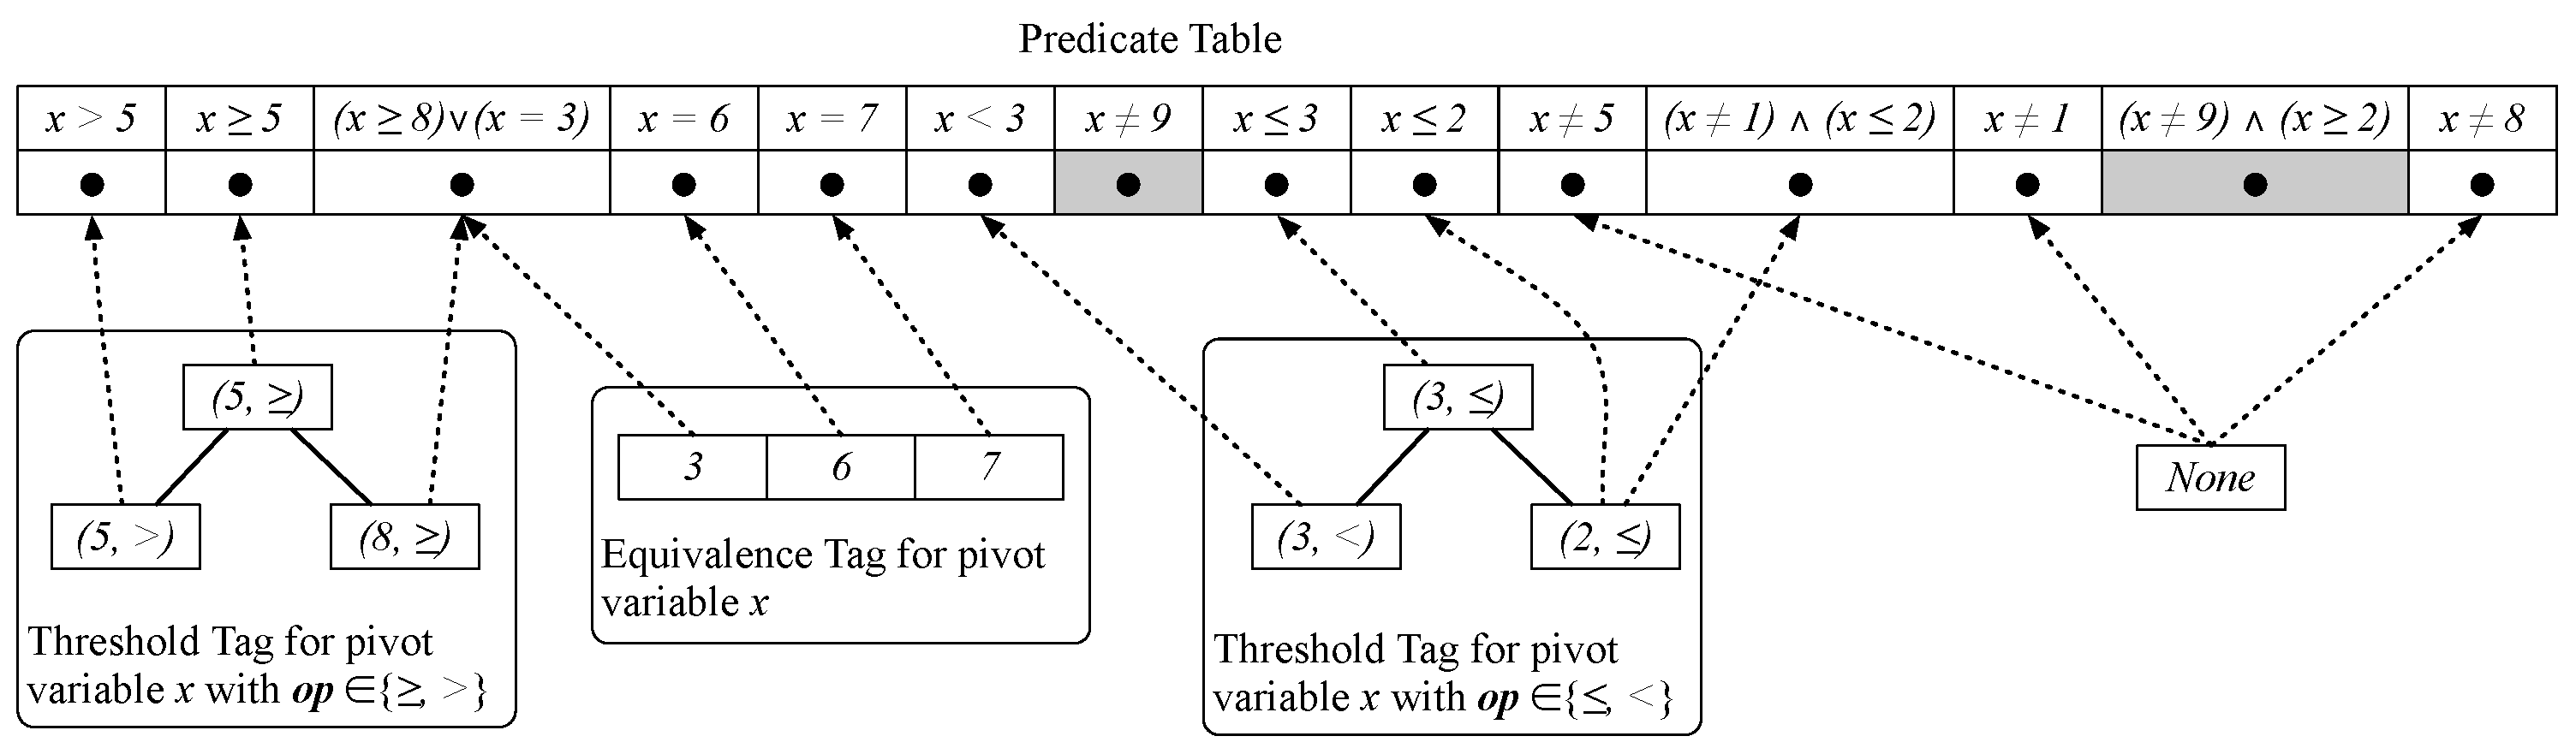
\includegraphics[width=180mm]{fig/manager.eps}
  \caption{A example of the condition manager in iMonitor}
  \label{fig:mgr}
\end{figure*}

A predicate must be removed from the tag once no thread waits on 
it to avoid unnecessary predicate evaluation. A threshold tag also needs to be
removed once it has no predicate. The reason is that 
we signal the root of the threshold predicate, a empty root 
will introduce overhead to find the next tag. 

Predicates may be reused. Instead  of removing those predicate with no waiting
thread, 
we move those predicate to an inactivate list. If they are used later, then we 
put them back. Otherwise, when the length of inactivate list exceeds some 
threshold, we remove the oldest predicates form the list.
%\clearpage


\section{Evaluations} \label{sec:eval}
%\subsection{Saturation}
\subsection{Environment}
All of the experiments were conducted on a machine with 16 
Intel(R) Xeon(R) X5560 CPUs and 64 GBs memory. 
%Four kinds of experiments were performed to evaluate the performances of the
%explicit-signal monitor with original Java and the implicit-signal monitor with
%iMonitor framework. 


\subsection{Signaling mechanisms}
The implementations using three different signaling mechanisms have been 
compared. 
\begin{description}
    \item[Explicit-signal] Using the original Java explicit-signal mechanism. 
    \item[iMonitor] Using the approach described in this paper. 
    \item[iMonitor-T] Using the approach described in this paper but excluding
        predicate tagging. 
    \item[Baseline] Using the implicit-signal mechanism which relying on only
        one condition variable. It calls signalAll all the time to check the
        predicates
\end{description}

\subsection{Test problems}
\begin{description}
    \item[Producer-Consumer (PC)] The traditional producer-consumer shown in 
        Fig.~\ref{fig:bb_exp}.
    \item[Producer-Consumer* (PC*)] The producer may produce $n$ elements a 
        time. In addition, the consumer may consume $n$ elements a time.
    \item[Readers/Writers (RW)] In the approach \cite{bh05}, a ticket is used
        to maintain the accessing order of readers and writers. Every reader
        and writer get a ticket number indicating its arrival order. Readers
        and writers are waiting on the monitor for their turn. 
    \item[Round-Robin Access Pattern (RR)] Every test thread accesses the
        monitor in round-robin order. 
\end{description}

The computing complexity is summarized in Tab.~\ref{tab:complexity}.
\begin{table}
   \centering
   \begin{tabular}{|c||c|c|c|c|}
      \hline 
         & PC & PC* & RW & RR \\
      \hline 
      explicit & $O(1)$ & $O(n)$ & $O(1)$ & $O(1)$ \\
      \hline 
      baseline & $O(1)$ & $O(n)$ & $O(n)$ & $O(n)$ \\
      \hline 
      iMonitor & $O(1)$ & $O(1)$ & $O(1)$ & $O(1)$ \\
      \hline 
   \end{tabular}
   \caption{The computing complexity}
   \label{tab:complexity}
\end{table}



%\subsection{Testbed}
%Fig.~\ref{fig:testbed} shows the experimental testbed \cite{bfc95}. 
%Every test thread has two state, monitor state and workload state. A thread
%query to access monitor in monitor state and perform its own job on workload
%state. The average response time of the monitor allows us evaluate the
%performance of different monitors. The first part of the experiments assume
%no workload for every thread. That is, every thread executes only monitor
%accessing calls with no other work. In the second part, we compared the
%performance under different workload.  
%\begin{figure}[ht!]
%  \centering
%  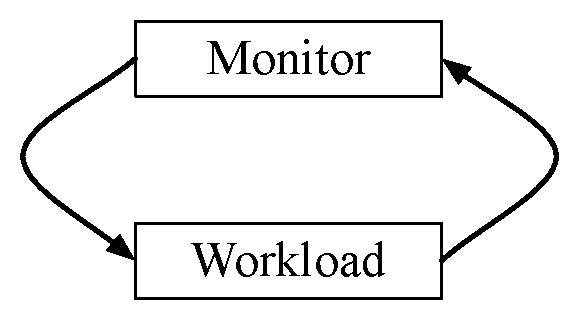
\includegraphics[width=40mm]{fig/testbed.eps}
%  \caption{The testbed}
%  \label{fig:testbed}
%\end{figure}
%
%\subsection{Saturation evaluation}
Fig.~\ref{fig:pc_eval} shows the results of producer-consumer problem. The
x-axis indicates the number of producers and consumers; the y-axis indicates the
runtime in seconds. Total 512000 $put$ and $take$ operations were executed by
all producers and consumers. As expected, than three signaling mechanisms have 
similar performance. This phenomenon can be explained as follows. There are 
only two waituntil statements with global predicates, $count > 0$ and 
$count < items.length$. Therefore, the complexity for signaling a thread in
implicit-signal mechanisms are also constant. Hence, the explicit-signal
mechanism is slightly more efficient than two other approaches. 
\begin{figure}[ht!]
  \centering
  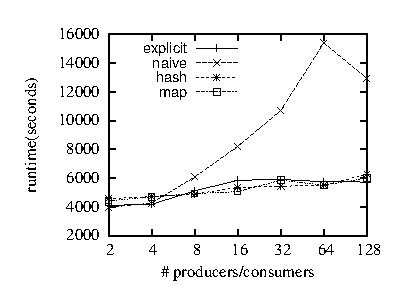
\includegraphics[width=80mm]{fig/pc.eps}
  \caption{The results of producer-consumer problem}
  \label{fig:pc_eval}
\end{figure}

%\begin{figure}
%  \centering
%  \subfloat[Explicit-Signal] {
%    \fbox{
%      \BUseVerbatim[fontsize=\footnotesize]{ExplicitNBoundedBuffer}
%    }
%    \label{subfig:rbb_exam_exp}
%  }
%  \\
%  \subfloat[Implicit-Signal] {
%    \fbox{
%      \BUseVerbatim[fontsize=\footnotesize]{iMonitorNBoundedBuffer}
%    }
%    \label{subfig:rbb_exam_imp}
%  }
%  \caption{Random Bounded-buffer example}
%  \label{fig:rbb_exp}
%\end{figure}
\begin{figure}[ht!]
  \centering
  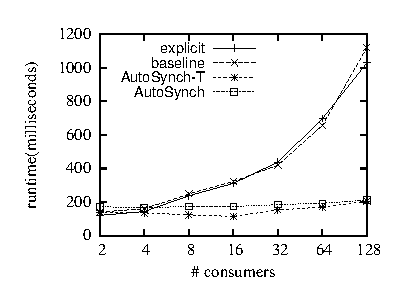
\includegraphics[width=80mm]{fig/rpc.eps}
  \caption{The results of random producer-consumer problem}
  \label{fig:rpc_eval}
\end{figure}

\begin{figure}[ht!]
  \centering
  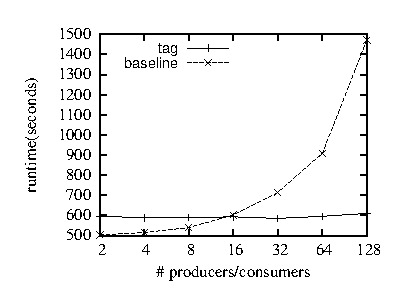
\includegraphics[width=80mm]{fig/rpch.eps}
  \caption{The results of random producer-consumer problem with comparing heap}
  \label{fig:rpc_eval}
\end{figure}

%Fig.~\ref{fig:rw_eval} shows the results of reader-writer problem. The
%x-axis indicates the number of readers and writers; the y-axis indicates the
%runtime in seconds. Total 1280 read/write operations were executed by all
%readers and writers. Since readers can read with each other at the same time.
%The runtime decreases as number of readers increases. Need to figure out why 
%explicit-signal approach is so slow in 1/5. Maybe the implementation? 
%
\begin{figure}[ht!]
  \centering
  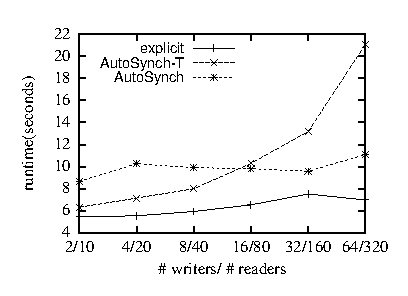
\includegraphics[width=80mm]{fig/trw.eps}
  \caption{The results of ticket reader-writer problem}
  \label{fig:rw_eval}
\end{figure}


%The dining philosophers problem is often used in computer science to describe 
%the synchronization issues. There are N philosophers siting around at a table 
%with a dish in front of them and a chopstick in between each philosopher. A 
%philosopher only think or eat. A philosopher needs to pick two chopsticks at the
%same time for eating and he does not put down a chopstick until he finishes 
%eating. If the chopstick is hold by another philosopher, then the philosopher 
%who want to eat must wait. In addition, a philosopher cannot eat forever, which
%means he will put down chopstick eventually. Every philosopher must be able to
%eat eventually if he is hungry. Figure 3. illustrate the experimental results
%of the dining philosophers problem. The x-axis depicts the runtime and the 
%y-axis describes the number of philosophers. As can be seen, three approaches 
%has the similar results. The implementations of Naive and N-condition are as 
%efficient as the implementation of explicit signal monitor. 
%
Fig.~\ref{fig:rr_eval} shows the results of round-robin access pattern. The
x-axis indicates the number of threads; the y-axis indicates the
runtime in seconds. In this set of experiments, threads are allowed to enter a
monitor in round-robin scheduling. Again, the results of N-Condition approach
are not shown because their performance is much worse than others. Total 
128000 operations were performed on the monitor. In this set
of experiment, the explicit-signal approach has an advantage since it can
explicitly to signal the next thread to enter the monitor. As can be seen, the
performance of explicit-signal approach is steady as the number of thread
increases. In comparison with our implicit-signal approaches, threads can only 
wait to enter the monitor. The runtime increases much as the number of thread 
increase in naive implementation. For the map approach, the performance is 
worse than the explicit-signal approach with a steady difference. 

\begin{figure}[ht!]
  \centering
  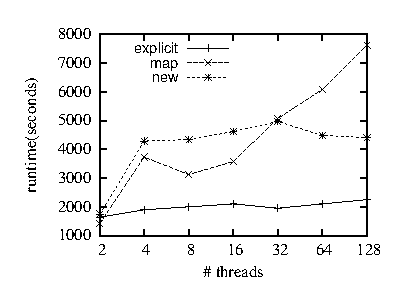
\includegraphics[width=80mm]{fig/rr.eps}
  \caption{The results of round-robin access pattern}
  \label{fig:rr_eval}
\end{figure}

%\subsection{Performance under different workload}
%\begin{figure}
%  \centering
%  \subfloat[Explicit-Signal] {
%    \fbox{
%      \BUseVerbatim[fontsize=\footnotesize]{ExplicitRoundRobinMonitor}
%    }
%    \label{subfig:rr_exam_exp}
%  }
%  \\
%  \subfloat[Implicit-Signal] {
%    \fbox{
%      \BUseVerbatim[fontsize=\footnotesize]{iMonitorRoundRobinMonitor}
%    }
%    \label{subfig:rr_exam_imp}
%  }
%  \caption{Round-Robin example}
%  \label{fig:rbb_exp}
%\end{figure}


%\subsection{Practical}
%Fig.~\ref{fig:dp_eval} shows the results of dining philosophers problem. The
%x-axis indicates the number of philosophers; the y-axis indicates the
%runtime in seconds. Every philosopher performed 100 eat operations with a
%randomly thinking time between 1 to 20 
%milliseconds. Fig.~\ref{fig:dp_eval} does not show the results of N-Condition 
%implementations since the results are much worse than other implementations. It
%takes around 10 minutes for 128 philosophers. The reason is that many waituntil
%statements with local predicate are used in this problem. Therefore, many
%condition variables are created and removed at runtime. As can be seen, the
%other three approaches have the similar results. This phenomenon can be
%explained as follows. The thinking time is much larger than the synchronization 
%time in the monitor. Therefore, the runtime is dominated by the thinking time.
%%These results suggest that if applications do not have many operations to access
%%a monitor, the performance will not have much difference in implicit-signal and
%%explicit-signal monitor.
%
%
%\begin{figure}[ht!]
%  \centering
%  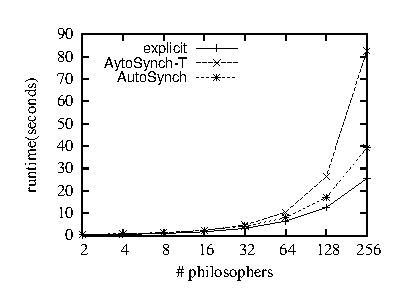
\includegraphics[width=80mm]{fig/dp.eps}
%  \caption{The results of dining philosophers problem}
%  \label{fig:dp_eval}
%\end{figure}

%\begin{figure}
%  \centering
%  \subfloat[Explicit-Signal] {
%    \fbox{
%      \BUseVerbatim[fontsize=\footnotesize]{ExplicitTicketReadersWriters}
%    }
%    \label{subfig:rw_exam_exp}
%  }
%  \\
%  \subfloat[Implicit-Signal] {
%    \fbox{
%      \BUseVerbatim[fontsize=\footnotesize]{iMonitorTicketReadersWriters}
%    }
%    \label{subfig:rw_exam_imp}
%  }
%  \caption{Random Bounded-buffer example}
%  \label{fig:rbb_exp}
%\end{figure}



\section{Related work} \label{sec:related}
\section{Conclusion} \label{sec:conclu}
In this paper, we propose the iMonitor framework that supports implicit-signal
mechanism with monitor class and waituntil statement. \dots

To evaluate the effectiveness of iMonitor, 

Using architecture info.

fairness

% use section* for acknowledgement








\appendix
%\section{Bounded-Buffer Code}
%\begin{figure*}[ht!]
%\begin{multicols}{2}
%    \begin{Verbatim}[fontsize=\footnotesize,gobble=8,frame=topline,
%            framesep=5mm,numbers=left,numbersep=2pt,
%            label=\fbox{\small\emph{Explicit-Signal}}]
%        class BoundedBuffer {
%          Object[] items;  
%          int putPtr, takePtr, count;
%          Lock mutex = new ReentrantLock();
%          Condition noSufficientSpace = mutex.newCondition();
%          Condition noSufficientItem = mutex.newCondition();
%          public BoundedBuffer(int n) {
%            items = new Object[n];
%            putPtr = takePtr = count = 0;
%          }
%          public void put(int n) {
%            mutex.lock();
%            while (n + count > items.length) {
%              noSufficientItem.signalAll();
%              noSufficientSpace.await();
%            }
%            for (int i = 0; i < n; ++i) {
%              items[putPtr++] = new Object();
%              if (putPtr == items.length) {
%                putPtr = 0;
%              }
%            }
%            count += n;
%            noSufficientItem.signalAll();
%            mutex.unlock();
%          }
%          public Object[] take(int n) {
%            mutex.lock();
%            while (count < n) {
%              noSufficientSpace.signalAll();
%              noSufficientItem.await();
%            }
%            Object[] ret = new Object[n];
%            for (int i = 0; i < n; ++i) {
%              ret[i] = items[takePtr++];
%              if (takePtr == items.length) {
%                takePtr = 0;
%              }
%            }
%            count -= n;
%            noSufficientSpace.signalAll();
%            mutex.unlock();
%            return ret;
%          }
%        }
%    \end{Verbatim}
%    \begin{Verbatim}[fontsize=\footnotesize,gobble=8,frame=lines,framesep=5mm,
%            numbers=left,numbersep=2pt,
%            label=\fbox{\small\emph{Implicit-Signal}}]
%        monitor class BoundedBuffer { 
%          Object[] items; 
%          int putPtr, takePtr, count; 
%          public void put(int n) { 
%            waituntil(count + n <= items.length); 
%            for (int i = 0; i < n; ++i) {
%              items[putPtr++] = new Object(); 
%              if (putPtr == items.length) { 
%                putPtr = 0; 
%              } 
%            }
%            count += n; 
%          } 
%          public Object[] take(int n) { 
%            waituntil(count >= n);
%            Object[] ret = new Object[n];
%            for (int i = 0; i < n; ++i) {
%              ret[i] = items[takePtr++]; 
%              if (takePtr == items.length) { 
%                takePtr = 0; 
%              }
%            }
%            count -= n;
%            return ret;
%          }
%        }
%    \end{Verbatim}
%\end{multicols}
%  \caption{Bounded-buffer example}
%  \label{fig:npc_exp}
%\end{figure*}
%\section{Readers/Writers Code}
%\begin{figure*}[ht!]
%\begin{multicols}{2}
%    \begin{Verbatim}[fontsize=\footnotesize,gobble=8,frame=topline,
%            framesep=5mm,numbers=left,numbersep=2pt,
%            label=\fbox{\small\emph{Explicit-Signal}}]
%        public class ReadersWritersMonitor {
%          int rcnt;
%          int ticket, serving;
%          Lock mutex = new ReentrantLock();
%          Map<Integer, Condition> mapCondition 
%              = new HashMap<Integer, Condition>();
%          public ReadersWritersMonitor() {
%            rcnt = ticket = serving = 0;
%          }
%          public void startRead() {
%            mutex.lock();
%            int myTicket = ticket;
%            ticket++;
%            Condition cond = mutex.newCondition();
%            mapCondition.put(myTicket, cond);
%            while (myTicket != serving) {
%              if (mapCondition.containsKey(serving)) {
%                 mapCondition.get(serving).signal();
%              }
%              cond.await();
%            }
%            mapCondition.remove(myTicket);
%            rcnt++;
%            serving++;
%            mutex.unlock();
%          }
%          public void endRead() {
%            mutex.lock();
%            rcnt--;
%            mutex.unlock();
%          }
%          public void startWrite() {
%            mutex.lock();
%            int myTicket = ticket;
%            ticket++;
%            Condition cond = mutex.newCondition();
%            mapCondition.put(myTicket, cond);
%            while (myTicket != serving || rcnt != 0) {
%              if (myTicket != serving &&
%                   mapCondition.containsKey(serving)) {
%                 mapCondition.get(serving).signal();
%              }
%              cond.await();
%            }
%            mapCondition.remove(myTicket);
%            mutex.unlock();
%          }
%          public void endWrite() {
%            mutex.lock();
%            serving++;
%            mutex.unlock();
%          }
%        }
%    \end{Verbatim}
%    \begin{Verbatim}[fontsize=\footnotesize,gobble=8,frame=lines,framesep=5mm,
%            numbers=left,numbersep=2pt,
%            label=\fbox{\small\emph{Implicit-Signal}}]
%        public monitor class ReadersWritersMonitor {
%          int rcnt;
%          int ticket, serving;
%          public ReadersWritersMonitor() {
%            rcnt = ticket = serving = 0;
%          }
%          public void startRead() {
%            int myTicket = ticket;
%            ticket++;
%            waituntil(myTicket == serving);
%            rcnt++;
%            serving++;
%          }
%          public void endRead() {
%            rcnt--;
%          }
%          public void startWrite() {
%            int myTicket = ticket;
%            ticket++; 
%            waituntil(myTicket == serving && rcnt == 0);
%          }
%          public void endWrite() {
%            serving++;
%          }
%        }
%    \end{Verbatim}
%\end{multicols}
%  \caption{Readers-writers example}
%  \label{fig:trw_exp}
%\end{figure*}
%\section{Round-Robin Monitor Code}
%\begin{figure}[ht!]
%    \begin{Verbatim}[fontsize=\footnotesize,gobble=8,frame=topline,
%            framesep=5mm,numbers=left,numbersep=2pt,
%            label=\fbox{\small\emph{Explicit-Signal}}]
%        public class RoundRobinMonitor{
%          int numProc;
%          int pid;
%          Lock mutex = new ReentrantLock();
%          Condition[] conds;
%          public RoundRobinMonitor(int n) {
%            numProc = n;
%            pid = 0;
%            Condition = new Condition[n];
%            for (int i = 0; i < n; i++) {
%              conds[i] = mutex.newCondition();
%            }
%          }
%          public void access(int myId) {
%            mutex.lock();
%            while (pid != myId) {
%              conds[pid].signal();
%              conds[myId].await();
%            }
%            pid = (pid + 1) % numProc;
%            conds[pid].signal();
%            mutex.unlock();
%          }
%        }
%    \end{Verbatim}
%    \begin{Verbatim}[fontsize=\footnotesize,gobble=8,frame=lines,framesep=5mm,
%            numbers=left,numbersep=2pt,
%            label=\fbox{\small\emph{Implicit-Signal}}]
%        public monitor class RoundRobinMonitor {
%          int numProc;
%          int pid;
%          public RoundRobinMonitor(int n) {
%            numProc = n;
%            pid = 0;
%          }
%          public void access(int myId) {
%            waituntil(pid == myId);
%            pid = (pid + 1) % numProc;
%          }
%        }
%    \end{Verbatim}
%  \caption{Round-Robin example}
%  \label{fig:rr_exp}
%\end{figure}
%
%
%\acks
%
%Acknowledgments, if needed.
%
%% We recommend abbrvnat bibliography style.
%
%\bibliographystyle{abbrvnat}
%
%% The bibliography should be embedded for final submission.
%
\begin{thebibliography}{}
\softraggedright

\bibitem {bfc95}
  P. A. Buhr, M. Fortier, and M. H. Coffin, \emph{Monitor Classification}. ACM 
  Computing Surveys, ACM, 27(1):63--107, 
  Nov. 2005.
  
\bibitem {bh05}
  P. A. Buhr and A. S. Harji, \emph{Implicit-signal monitors}. ACM 
  Transactions on Programming Languages and Systems ACM, 27(6):1270--1343, 
  Nov. 2005.

\bibitem {han75}
  P. B. Hansen, \emph{The Programming language concurrent Pascal}. IEEE
  Trans.~Software Engineering, 1(2), 149--207, 1975.

\bibitem {hoa74}
  C. A. R. Hoare, \emph{Monitors: an operating system structuring concept}. 
  Commun.~ACM 17, 10(Oct. 1974), 549--557.



\end{thebibliography}
\end{document}
